% !Mode:: "TeX:UTF-8"
% !TEX program  = xelatex
\documentclass[a4paper]{article}
\usepackage{ctex}
\usepackage[left=1.5cm, right=1.5cm, top=1.5cm, bottom=1.5cm]{geometry} %页边距
\usepackage{helvet}
\usepackage{amsmath, amsfonts, amssymb} % 数学公式、符号
\usepackage[english]{babel}
\usepackage{graphicx}   % 图片
\usepackage{url}        % 超链接
\usepackage{bm}         % 加粗方程字体
\usepackage{multirow}
\usepackage{booktabs}
\usepackage{tikz}%调用宏包tikz
\usepackage{circuitikz}%调用宏包circuitikz
\usepackage{enumerate}
\usepackage{algorithm}
\usepackage{algorithmicx}
\usepackage{algpseudocode}
\usepackage{graphicx}
\usepackage[hidelinks]{hyperref}
\usepackage{listings}
\usepackage{textcomp}
\usepackage{multicol}
\usepackage[backend=biber,style=numeric,sorting=none]{biblatex}
\addbibresource{reference.bib}

% Python listing
\newcommand\pythonstyle{\lstset{
language=Python,
basicstyle=\sffamily,
keywordstyle=\textbf,
commentstyle=\color{blue},
showstringspaces=false, 
numbers=left }}
% Python environment
\lstnewenvironment{python}[1][]{
\pythonstyle \lstset{#1} }{}

\newcommand{\threemetrics}[3]{\multirow{3}{*}{\shortstack[c]{$\textcolor{orange}{#1}$\\$\textcolor{blue}{#2}$\\$\textcolor{green}{#3}$}}}
\newcommand{\twometrics}[2]{\multirow{2}{*}{\shortstack[c]{$\textcolor{blue}{#1}$\\$\textcolor{green}{#2}$}}}

\renewcommand{\algorithmicrequire}{ \textbf{Input:}}       
\renewcommand{\algorithmicensure}{ \textbf{Output:}} 
%算法格式
\usepackage{subfigure}
\usepackage{fancyhdr} %设置页眉、页脚
\usepackage{gensymb}

\pagestyle{fancy}
\lhead{MiniProject 3: Image Unpermutation, AI3607 Deep Learning and Its Application}
\chead{}
\rhead{蒋伟, 520030910149}
\lfoot{}
\cfoot{\thepage}
\rfoot{全部实验结果详见各 \texttt{checkpoint} 目录。}


\usepackage{ifthen}
\usepackage{xifthen}

\newcommand{\dom}[1]{\mathop{\mathrm{dom}}\left(#1\right)}
\newcommand{\rng}[1]{\mathop{\mathrm{rng}}\left(#1\right)}
\newcommand{\preimg}[2][]{ \ifthenelse{\isempty{#1}}
  {\mathop{\mathrm{preimage}}\left(#2\right)}
  {\mathop{\mathrm{preimage}}_{#1}\left(#2\right)} }
\newcommand{\set}[1]{\left\{#1\right\}}

\newenvironment{proof}{{\par\noindent\it Proof.}\quad\par}{\hfill $\square$\par}  

\begin{document}
\section{目标任务}
    %\item 将输入图片分割为 $N$ 张子图片打乱输入,并将他们的正确排列作为输出,输出格式采用排列阵 $P$,第 $i$ 行第 $j$ 列若为 $1$ 则代表图片 $i$ 排在位置 $j$,每行每列只有唯一一个元素为 $1$。
    设计一套针对图片拼接的神经网络,并尝试能否将其作为一种预训练来辅助作业二中的图片分类任务。
    %即对每一个子图片过一个 CNN,将得到的特征进行拼接后过若干全连接网络后得到一个 N x N 的矩阵,通过 Sinkhorn 算法使其变成双随机矩阵 Q(每行每列的和固定为 1)作为神经网络的预测值。最后将预测值 Q(双随机矩阵)与真值 P(排列阵)作 Loss 后用于更新神经网络。

\section{图片拼接数据集(CIFAR-10 PERMutation)}
在 CIFAR-10 数据集中,如图 \ref{fig:1} 将一张图片拆分为左上、右上、左下、右下(对应位置标签 $0, 1, 2, 3$)四个等大子图,并随机排列。目标为重排的正确位置标签。可以将此图片拼接问题看成分类问题,类别就是位置。

\begin{figure}[H]
    \centering
    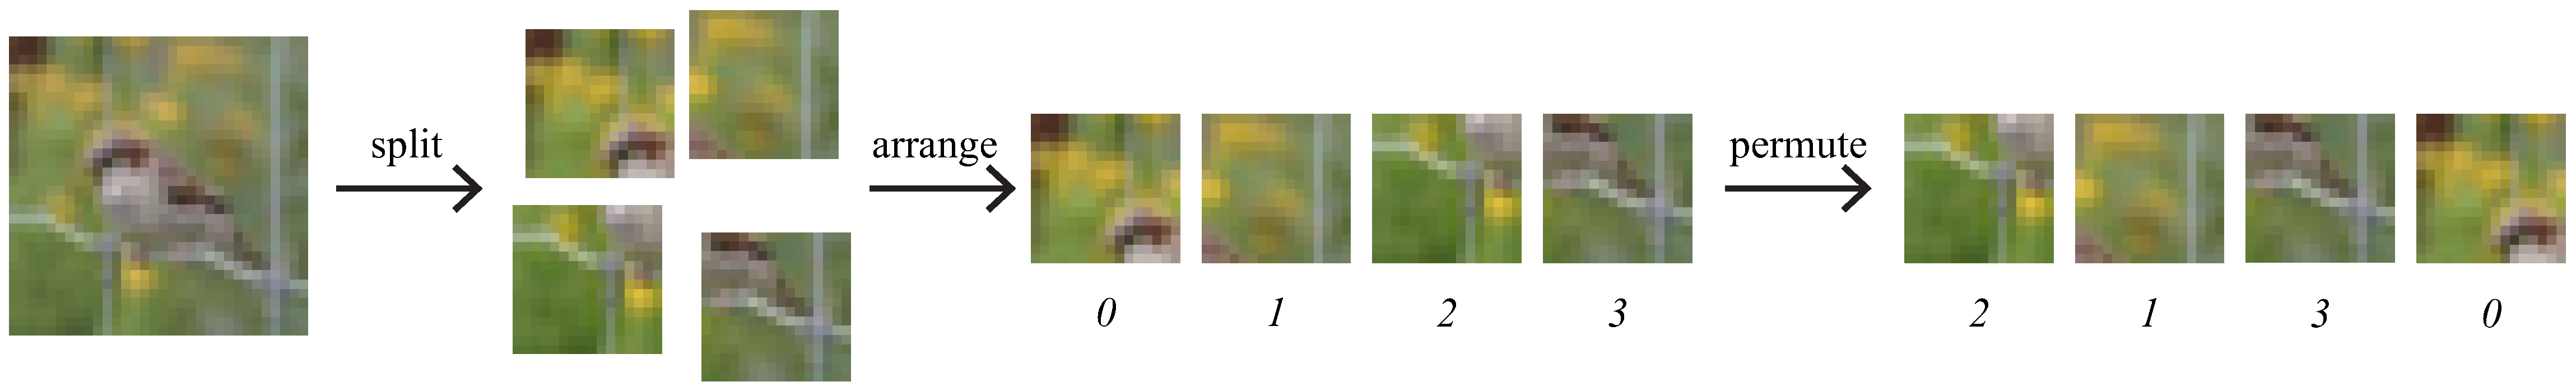
\includegraphics[width=0.95\linewidth]{images/data.eps}
    
    \caption{Illustration of splitting one image into 4 patches and permuting them, as the dataset does.}
    \label{fig:1}
\end{figure}

\section{CIFAR-10 PERM 数据集图片拼接}
\subsection{网络结构}
参考 DeepPermNet \cite{deeppermnet} 的模型范式,我采用了平行卷积特征提取、多子图特征聚合、双随机矩阵生成的流程。

卷积提取网络的架构与作业二中的 Simple Classifier 前几层类似,称为 Simple Extractor。特别地,Simple Extractor 进行了尺寸不变 padding 来保留对拼接可能更重要的边缘信息。而后续则使用与 DeepPermNet 中各维度都相同的线性层作为特征聚合器(Aggregator)。其中,第一层线性层将数据维度增大,从而快速,乃至带来冗余地融合多子图信息。最后通过 Sinkhorn \cite{sinkhorn1, sinkhorn2} 算法进行归一化得到双随机矩阵(每行每列的和固定为 $1$),作为预测值输出。具体模型结构和运行管线如图 \ref{fig:2}。

\begin{figure}[H]
    \centering
    \includegraphics[width=0.85\linewidth]{images/archi.eps}
    \caption{Pipeline and architecture of the method.}
    \label{fig:2}
\end{figure}

\subsection{训练目标}
如前所述,本任务可以看作是分类任务,分类的对象是子图,类别是子图的位置。此时的直观想法就是对每张子图计算交叉熵损失进行加和。但实际上,我们计算得到的双随机矩阵 $Q$ 不仅表示每个子图所属位置的概率分布(从每行看),还可以理解为每个位置应放子图的概率分布(从每列看)。换言之,双随机矩阵表达了子图和位置两个随机变量的联合分布。因此,对于训练的目标还需要进一步讨论。

对于联合分布 $p(X,Y)$,有联合熵(joint entropy)
\[
    H(X,Y) = -\sum_x \sum_y p(x, y) \ln p(x,y),
\]
而此时代入真实概率分布 $p(X,Y)$ 和预测概率分布 $q(X, Y)$,就能得到联合分布的交叉熵
\[
    H(p,q) = \mathbf{E}_p\left[-\ln q(x,y)\right] = -\sum_x \sum_y p(x, y) \ln q(x,y).
\]

回顾对每张子图计算交叉熵损失并求和,有
\[
    H(p(x, \cdot), q(x, \cdot)) =  -\sum_y p(x, y) \ln q(x,y),
\]
\[
    \sum_x H(p(x, \cdot), q(x, \cdot)) =  -\sum_x\sum_y p(x, y) \ln q(x,y) = H(p,q),
\]
因此,在双随机矩阵引入的(或假设的)概率先验下,直接计算每张子图的交叉熵损失并进行加和,就等价于计算联合分布的交叉熵,是符合概率学的损失函数定义方式。

特别地,如果不进行和为一的归一化,损失函数的惩罚也可以引起正确预测“概率”的增长,得到较好的训练结果。在使用梯度性质不佳的归一化导致结果较差时,可以尝试放弃概率可解释性,直接使用未归一化的输出进行损失计算。此时得到的损失只具有训练过程中的相对意义。

\section{使用预训练 Simple Extractor 的图片分类}
由于图片尺寸和输出尺寸有不同,且模型的前部能够提取具有泛用能力的特征,而后部往往倾向于整合任务相关的特征,我选择只取用 Simple Extractor 的预训练参数,并对提取得到的特征使用新训练的神经网络进行处理分析。
\subsection{网络结构}

我选择了两种代表性的结构思路进行设计,第一种与作业三的网络结构更相似,第二种则更类似作业二的网络结构。
\subsubsection{Patched Classifier}
一种直接的想法是沿用作业三中的子图结构,从而保证预训练参数与数据之间的适应性,结构见图\ref{fig:3a}。这种结构不能完整地学习图片的全局信息,且在特征整合上也设计得较为简单,因此在分类任务中表现并不好。
\subsubsection{Two-stage Classifier}
另一种思路是直接将 Simple Extractor 前几层卷积层作为全图的卷积层使用,之后使用线性层直到最终输出预测,结构见图\ref{fig:3b}。这种方法的可行性在于尽管图片大小不同,卷积核相对于整张图片的尺度是在两个任务中不变的,因此原先用于处理子图的网络同样能用于处理整张图片。值得一提的是,在本结构中,对提取得到的特征没有采取升维操作,而是仿照 Simple Classifier 的网络结构设计了 $256-96-10$ 的逐步降维线性层。


\begin{figure}[H]
    \centering
    \subfigure[Patched Classifier.]{
        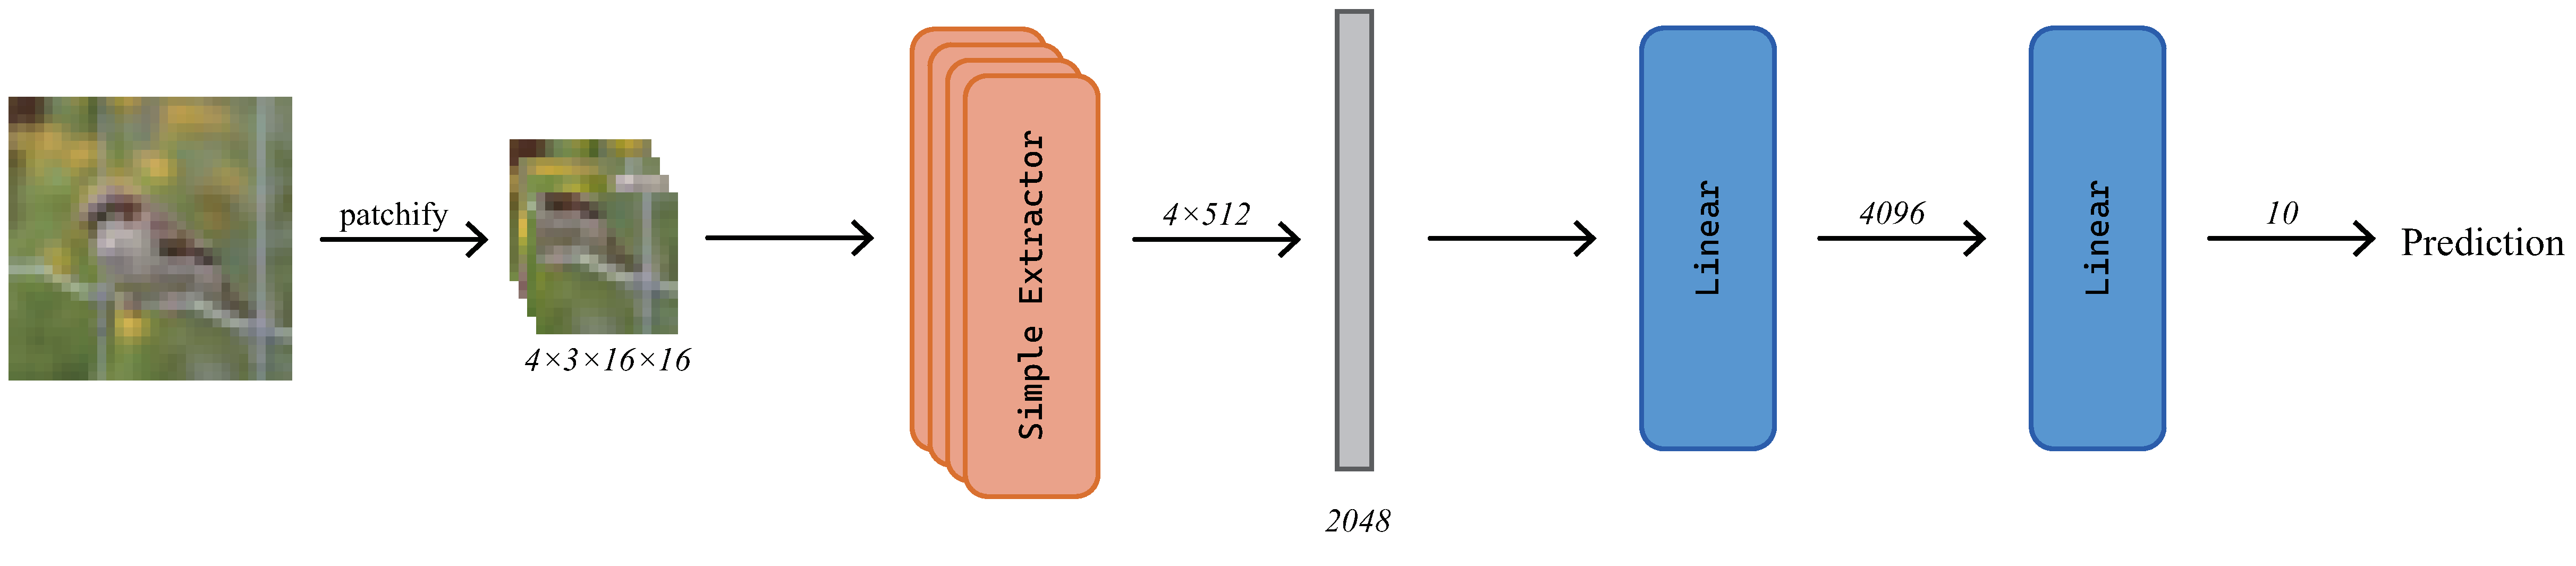
\includegraphics[width=0.8\linewidth]{images/patched.eps}
        \label{fig:3a}
    }
    
    \subfigure[Two-stage Classifier. SE is short for Simple Extractor.]{
        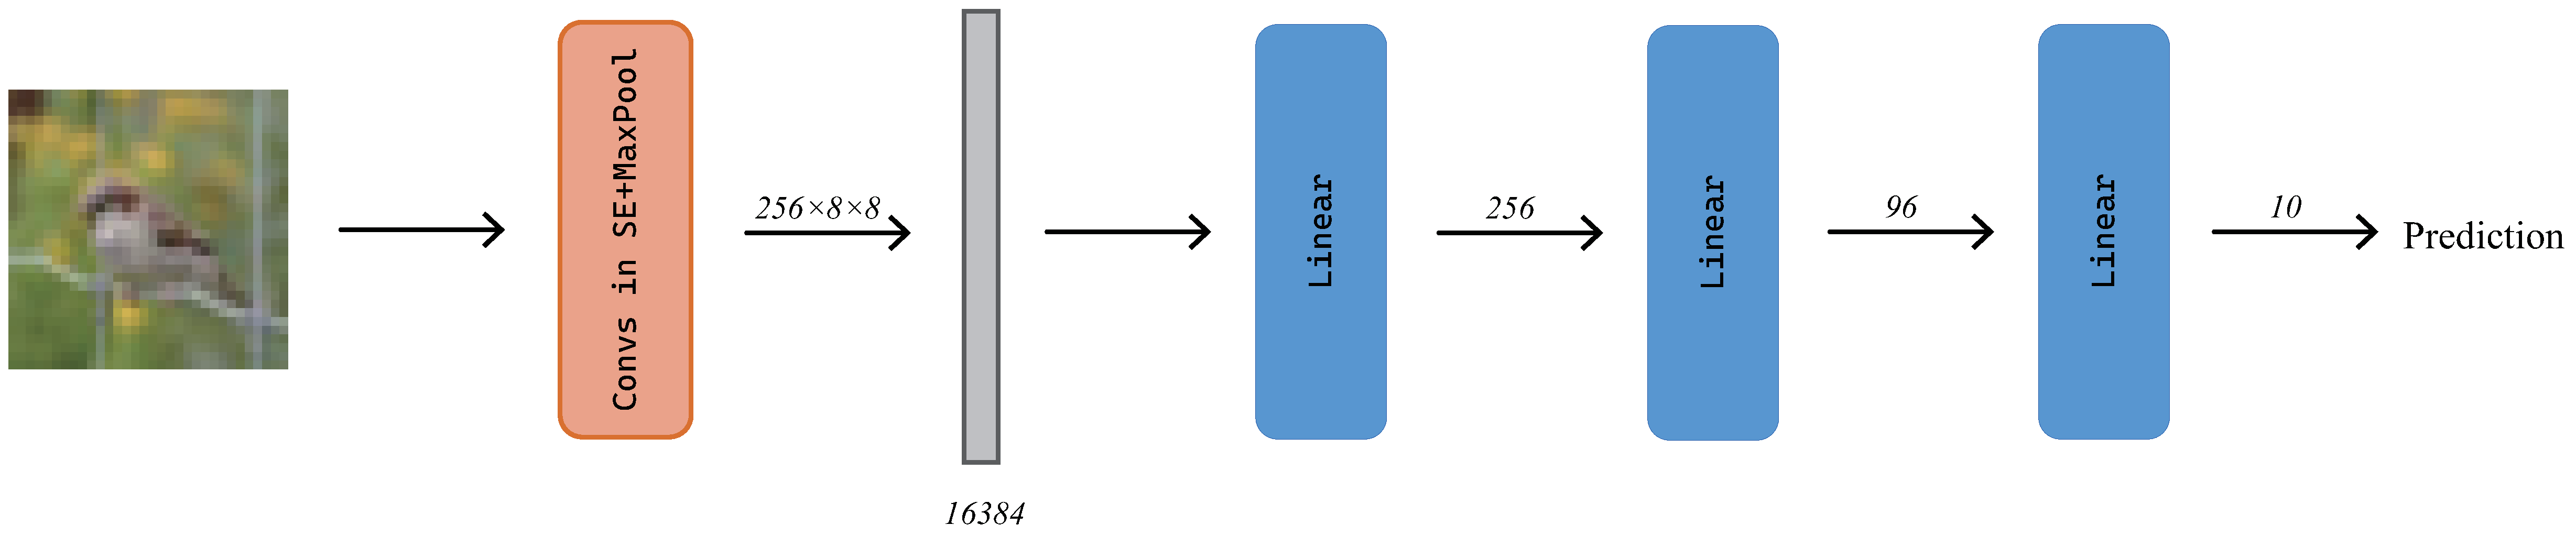
\includegraphics[width=0.8\linewidth]{images/two-stage.eps}
        \label{fig:3b}
    }
    \caption{Architectures of classifiers with pretrained Simple Extractor.}
\end{figure}


\subsection{对抗过拟合}
训练过程中出现明显过拟合,亦可使用数据增强和 weight decay 来增加模型的鲁棒性、泛化性,甚至使得模型在未增强的测试集上的准确率高于训练准确率。

\section{实验结果}
实验结果如表 \ref{tab:1}, \ref{tab:2} 所示。有趣的是,与 DeepPermNet \cite{deeppermnet} 的结果不同,在本实验的设置下,不使用计算略复杂的 Sinkhorn 反而既提升了训练速度又提高了模型表现。在不必输出预测概率时,或许这是更好的选择。

\begin{table}[H]
    \centering
    \begin{tabular}{cccccccccccccccc}
        \hline
        &\multicolumn{3}{c}{With Sinkhorn}&\multicolumn{7}{c}{Without Sinkhorn}\\
        Model           &Pure&WD1&C+F.3&            Pure&WD.3&WD.5&WD1&WD3&WD5&WD6&WD7&WD10&C&C+F.3&C+F.3+WD1\\
        \hline
        Train Loss      &$0.7691$&$0.7865$&$0.8177 $&     $0.0038 $&$0.0097 $&$0.0140 $&$0.0254 $&$0.0675 $&$0.1133 $&$0.1348$&$0.1574$&$0.2268 $\\
        Loss            &$0.8628$&$0.8731$&$0.8160 $&     $0.5168 $&$0.4064 $&$0.3741 $&$0.3314 $&$0.2809 $&$0.2689 $&$0.2691$&$0.2721$&$0.3273 $\\
        Acc.            &$0.8802$&$0.8773$&$0.9317 $&     $0.8880 $&$0.8883 $&$0.8884 $&$0.8921 $&$0.8965 $&$0.8996 $&$0.9002$&$0.8994$&$0.8785 $\\
        \hline
    \end{tabular}
    \caption{Result of our image concatenator in aid of anti-overfitting methods. WDX, C, and F.X stand for weight decay of $Xe-3$, random crop, and random flip with rate $0.X$, respectively. Train losses, test losses, and test accuracies are reported.}
    \label{tab:1}
\end{table}

\begin{table}[H]
    \centering
    \begin{tabular}{ccccccc}
        \hline
        &\multicolumn{2}{c}{From Scratch}&\multicolumn{2}{c}{Pretrained}&\multicolumn{2}{c}{Finetune}\\
        Model&Two-stage&Patched&Two-stage&Patched&Two-stage&Patched\\
        \hline
        Loss\\
        Acc.\\
        \hline

    \end{tabular}
    \caption{Result of classifiers with Simple Extractor on CIFAR-10. Weights from .}
    \label{tab:2}
\end{table}


\section{训练细节}

学习率 $3e-4$ 衰减 $0.8$。不使用 weight decay。batch size $1024$,共训练 $5,000,000$ 迭代。从第 $50,000$ 次起每 $200,000$ 次迭代学习率衰减。数据增强不启用;若启用,方式为随机翻转和随机裁剪。

对分类任务:学习率 $1e-2$ 衰减 $0.5$。weight decay $1e-3$。

\end{document}